\documentclass[a4paper,12pt]{article} 
\setcounter{page}{2}
\usepackage{cmap}          
\usepackage{mathtext}         
\usepackage[T2A]{fontenc} %Указывает, какую кодировку шрифта(кириллицы)   
\usepackage[utf8]{inputenc}  
\usepackage[english,russian]{babel} %языки, правила расстановки переносов  
\usepackage{amsmath,amsfonts,amssymb,amsthm,mathtools} %доп.символы
\usepackage{icomma} % для отображения запятой как разделителя целой и дробной частей числа
\usepackage{euscript} %рукописный шрифт  
\usepackage{mathrsfs}  
\usepackage{tikz} % использование векторной графики
\usepackage{graphicx} 
\graphicspath{{pictures/}} 
\setlength\fboxsep{3pt} 
\setlength\fboxrule{1pt} 
\usepackage{wrapfig} % текст вокруг фигуры
\usepackage{indentfirst} %позволяет делать в первом абзаце после заголовка абзацный отступ
\usepackage{geometry}
\geometry{left=3.5cm}
\geometry{right=1.0cm}
\geometry{top=2.0cm}
\geometry{bottom=2.0cm}
\linespread{1.5} %разброс строк 
\usepackage{listings} %можно добавлять код




            
\begin{document}
  \begin{titlepage}  
\begin{minipage}{0.2\textwidth}
\end{minipage}
\begin{minipage}{0.8\textwidth}
  \centering\textbf{«МОСКОВСКИЙ АВТОМОБИЛЬНО-ДОРОЖНЫЙ ГОСУДАРСТВЕННЫЙ ТЕХНИЧЕСКИЙ УНИВЕРСИТЕТ (МАДИ)»}
\end{minipage}
\\  
\vspace{4cm}

\centering Кафедра «Высшая математика»
\\


\centering\textbf{КУРСОВАЯ РАБОТА} %жирный шрифт
\\

\centering \textbf{на тему:} «Исследование характеристик транспортного потока по видеоряду с камеры наблюдения»
\\

\centering \textbf{по дисциплине:} «Прикладное программирование и пакеты программ»
\\

\vspace{2cm}

\begin{flushright}
\begin{table}[h!]
  \begin{tabular}{lllllllllllllllllllllll}
    &  &  &  &  &  &  &  &  &  &  &  &  &  &  &  &  &  &  &  &  &  & \textbf{Выполнил}                       \\
    &  &  &  &  &  &  &  &  &  &  &  &  &  &  &  &  &  &  &  &  &  & Учебная группа: 1бПМ2                    \\
    &  &  &  &  &  &  &  &  &  &  &  &  &  &  &  &  &  &  &  &  &  &
    Пасечник Александра Викторовна\\
    &  &  &  &  &  &  &  &  &  &  &  &  &  &  &  &  &  &  &  &  &  & Подпись \makebox[3cm]{\hrulefill}                    \\
    &  &  &  &  &  &  &  &  &  &  &  &  &  &  &  &  &  &  &  &  &  & \textbf{Руководитель:} \\
    &  &  &  &  &  &  &  &  &  &  &  &  &  &  &  &  &  &  &  &  &  & Старший преподаватель                   \\
    &  &  &  &  &  &  &  &  &  &  &  &  &  &  &  &  &  &  &  &  &  & Доткулова Анастасия Сергеевна           \\
    &  &  &  &  &  &  &  &  &  &  &  &  &  &  &  &  &  &  &  &  &  & Подпись \makebox[3cm]{\hrulefill}                    
  \end{tabular}
\end{table}
\end{flushright}

\vspace{0.5cm}



\vspace{2cm}
\centering Москва 2022 г.
\end{titlepage}

\newpage
\tableofcontents


\newpage
\section{Введение}  
Современные технологии позволяют решать проблемы, возникающие с транспортными средствами.

В данной работе поставлена задача анализа автомобильного потока, его интенсивности.
Для ее решения будут рассмотрены различные средства мониторинга дорожно-транспортной инфраструктуры путём обработки видеопотока.

Видеопоток — это временная последовательность кадров определенного формата, закодированная в битовый поток.
Видеоряд — это последовательность сменяющих друг друга картинок. 
Интенсивность потока – это количество транспортных средств, проходящих в единицу времени через заданное сечение. 

\subsection{Исходные данные}
На вход работы алгоритма подаётся видеофайл формата «*.mp4»  продолжительностью 37 секунд. Файл взят с камеры, установленной по адресу г. Москва, Ленинградский проспект, 64. Дата и время записи: 8 февраля 2022 года, 16:14. Погодные условия: пасмурно, без осадков. 

\newpage

\section{Цель и задачи}  
\subsection{Цель}  
Исследовать видеопоток и оценить основные характеристики транспортного потока по видеоряду, полученному из окна аудитории «МАДИ», которое выходит на Ленинградское шоссе. Требуется создание следующего функционала:\\
1.	Выбор видеофайла для исследования из интерфейса приложения;\\
2.	Расположение детекторов на видео;\\
3.	Вывод основных характеристик транспортного потока.\\
\subsection{Задачи} 
\noindent 1. Получить видеопоток;\\
2. Разбить видеопоток на кадры;\\
3. Конвертировать кадры в градацию серого;\\
4. Выставить детекторы, количество детекторов не ограничено;\\
5. Вычислить значение среднего цвета каждого кадра в выбранной области для каждого детектора;\\
6. Сравнить значение средних цветов между собой;\\
7. Построить график по среднему цвету для каждого детектора;\\
8. Построить бинаризованный график для каждого детектора;\\
9. Построить график изменения среднего цвета по времени для каждого детектора;\\
10. Вычислить интенсивность потока и подсчитать количество автомобилей (для каждого детектора).


\subsection{Актуальность работы}
Актуальность работы заключается в том, что мы можем считать характеристики транспортного потока, измерять интенсивность и плотность потока, моделировать ситуации на дороге. 

\newpage

\section{Основная часть}

\subsection{Часть Турбина В.М.}

Для работы используется заранее подготовленная запись видеопотока, на котором будет проводиться определение основных характеристик транспортного потока. 
Установка детекторов происходит с помощью одного клика мышки.


Видеоряд был записан на камеру, установленной в университете "МАДИ", аудитория № 441. После съемки видеофайл с расширением .mp4 сохраняется на персональный компьютер.Видеофайл считывается с помощью функции VideoCapture.

\begin{figure}[h!]
  \begin{center}
      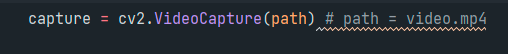
\includegraphics[width=0.8\linewidth]{openfile}
      \caption{Чтение видеофайла} 
      \label{} 
  \end{center} 
\end{figure}

Затем происходит покадровая обработка видео. Программа переводит кадры в серый цвет с помощью cv2.cvtColor.
Пользователю предлагается выбрать расположение виртуальных детекторов. Машины пересекают детектор. Размер детектора можно задать в коде(по умолчанию 10x10), а расположение отображено зелёным квадратом.

\begin{figure}[h!]
  \begin{center}
      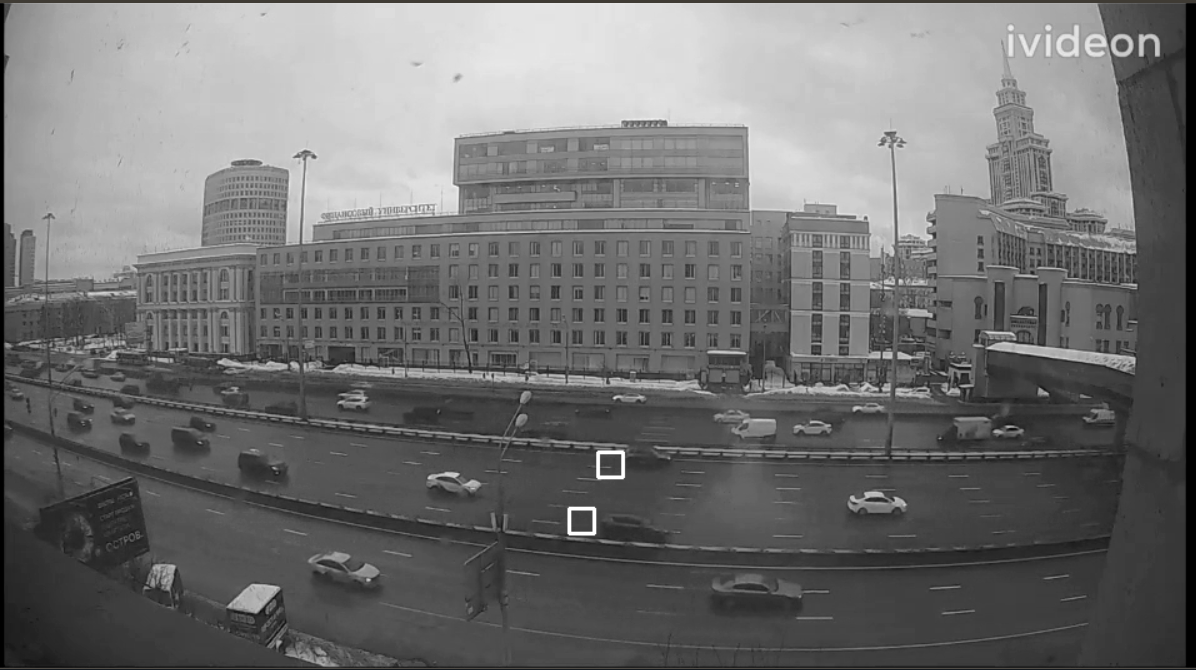
\includegraphics[width=0.8\linewidth]{detectors}
      \caption{Расстановка детекторов и перевод видео в серый цвет} 
      \label{} 
  \end{center} 
\end{figure}

Программа раставляют детекторы с помощи специальной функции представленной на рисунке 2.

\begin{figure}[h!]
  \begin{center}
      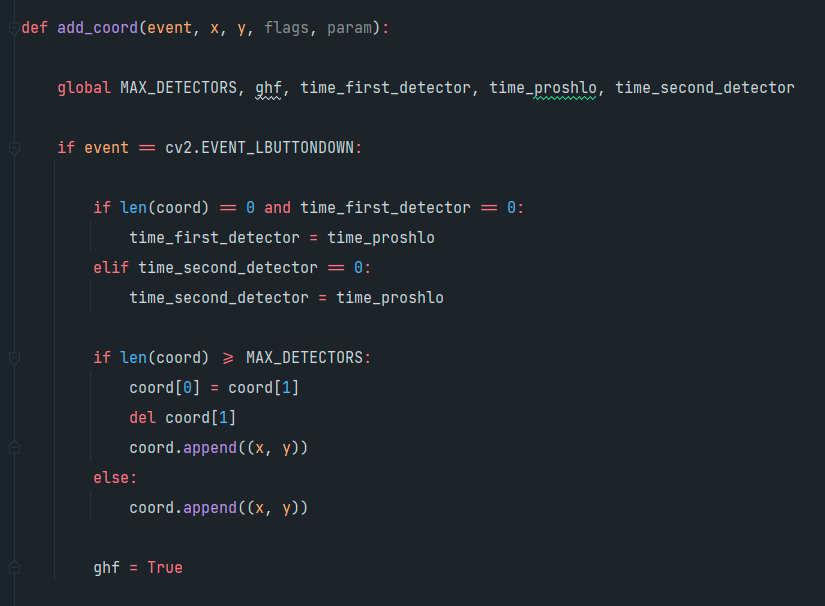
\includegraphics[width=0.8\linewidth]{callback}
      \caption{Функция, срабатывающая при нажатии ЛКМ} 
      \label{} 
  \end{center} 
\end{figure}

Далее программа вычисляет средний цвет серого в каждом из детекторов.

\begin{figure}[h!]
  \begin{center}
      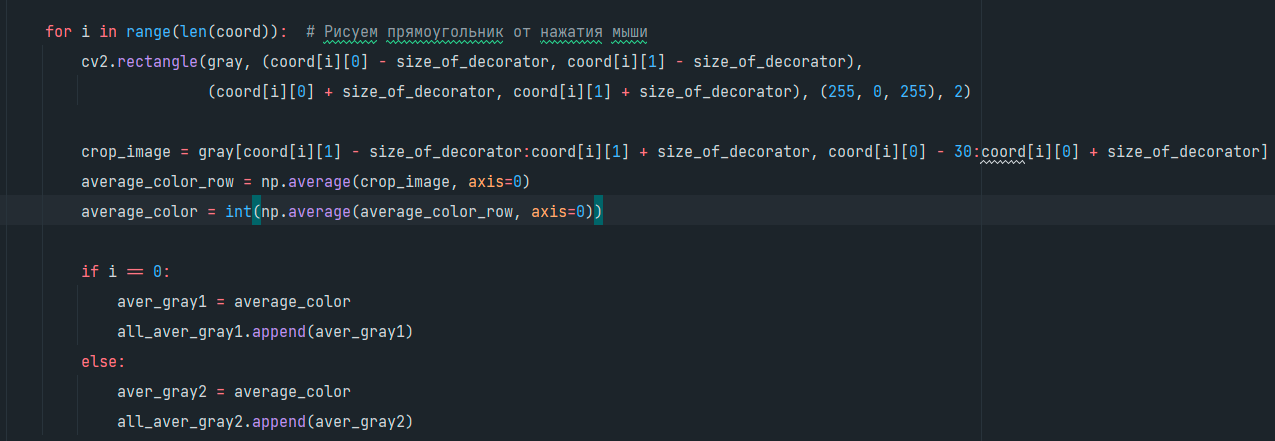
\includegraphics[width=0.8\linewidth]{grayscale}
      \caption{Подсчёт среднего значения серого цвета} 
      \label{} 
  \end{center} 
\end{figure}

\newpage

\subsection{Часть Пасечник А. В.}
Следующим шагом программа считатет для каждого кадра значение среднего серого цвета в детекторах и заносит эти данные в соответствующий вектор(allavergrey).
После окончания работы алгоритма программа выводит график среднего значения цвета. 

\begin{figure}[h!]
  \begin{center}
      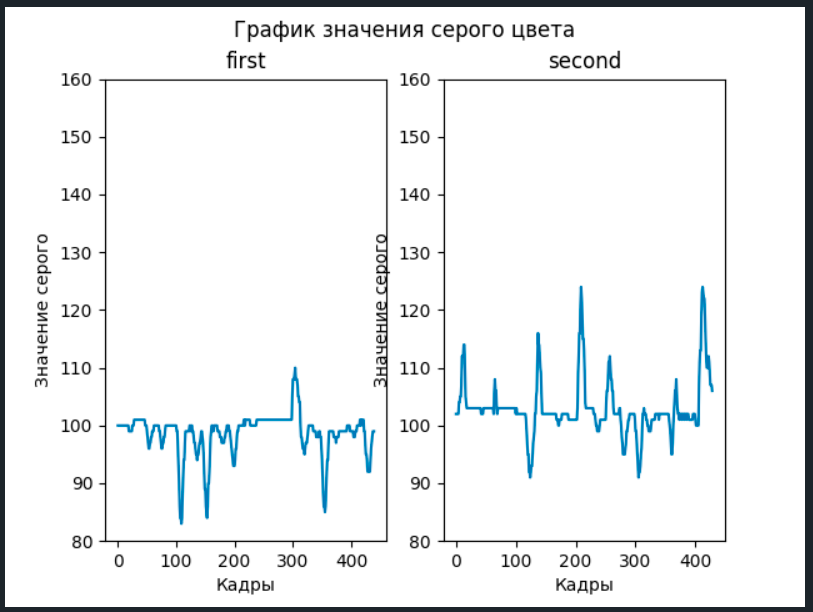
\includegraphics[width=0.8\linewidth]{gray_scale_graphic}
      \caption{График по среднему значению цвета для каждого детектора} 
      \label{} 
  \end{center} 
\end{figure}

Так как в программе стоит задержка 60 мс перед каждым кадром, то достаточно просто сделать график среднего значения серого цвета в каждом детекторе, если засекать время появления каждого из детекторов.
Время засекается в функции, реагирующей на нажатие мышки.

\begin{figure}[h!]
  \begin{center}
      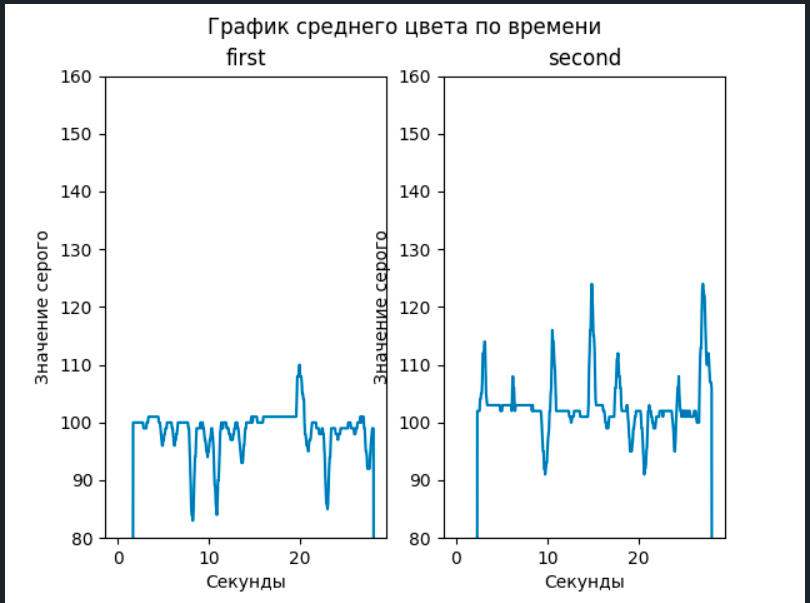
\includegraphics[width=0.8\linewidth]{time_grayscale}
      \caption{График по среднему значению цвета для каждого детектора в секунды} 
      \label{} 
  \end{center} 
\end{figure}

\newpage

\subsection{Часть Тумасова В. Д.}

Программа сравнивает значения среднего серого цвета предыдущего и текущего кадров. Если разница составляет более 3 процентов, то функция возвращает значение 1, если менее 3 процентов - 0. 

\begin{figure}[h!]
  \begin{center}
      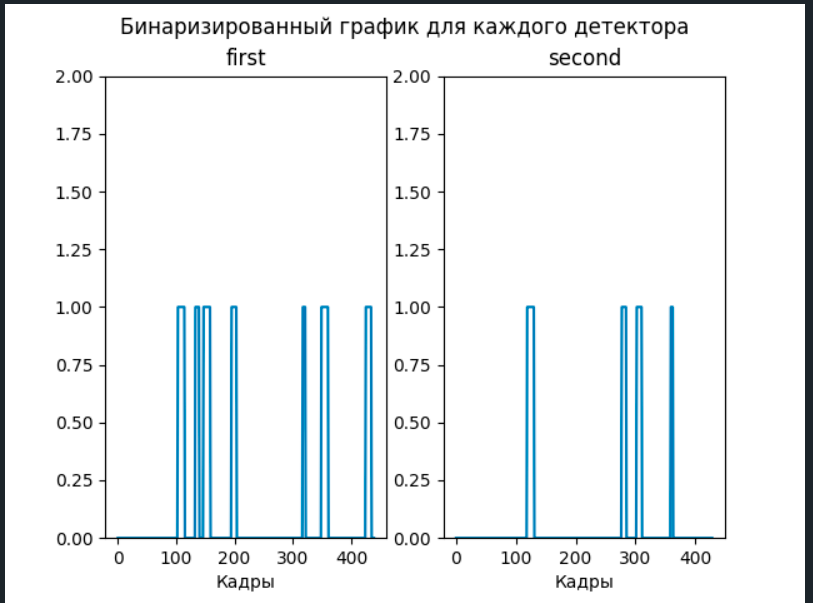
\includegraphics[width=0.8\linewidth]{bin_graph}
      \caption{Бинаризованный график} 
      \label{} 
  \end{center} 
\end{figure}

Функцию реализующая дискретизацию графика выглядит следующим образом(рис.8).

\begin{figure}[h!]
  \begin{center}
      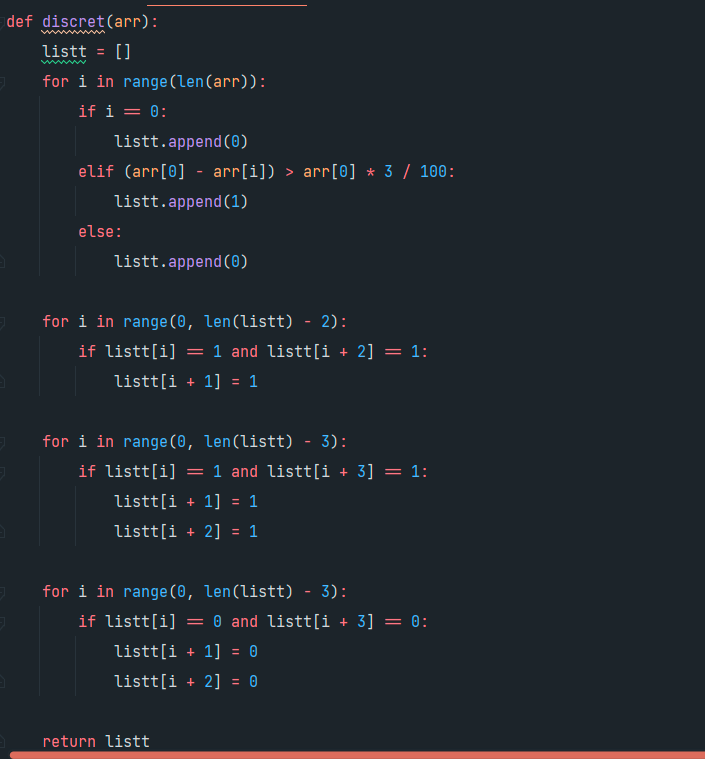
\includegraphics[width=0.8\linewidth]{bin_func}
      \caption{Функция дискретизации} 
      \label{} 
  \end{center} 
\end{figure}

\newpage

По результатам бинаризованного графика, изображенного на рис.7 можно судить о количестве автомобилей, пересекших детектор. Так, при значении равным 1 – автотранспортное средство есть в кадре, при 0 – отсутствует.
Бинаризированный график показан на рис.8.

Далее программа высчитывает количество машин в каждом из детекторов. Результат приведён на рис.9.

\begin{figure}[h!]
  \begin{center}
      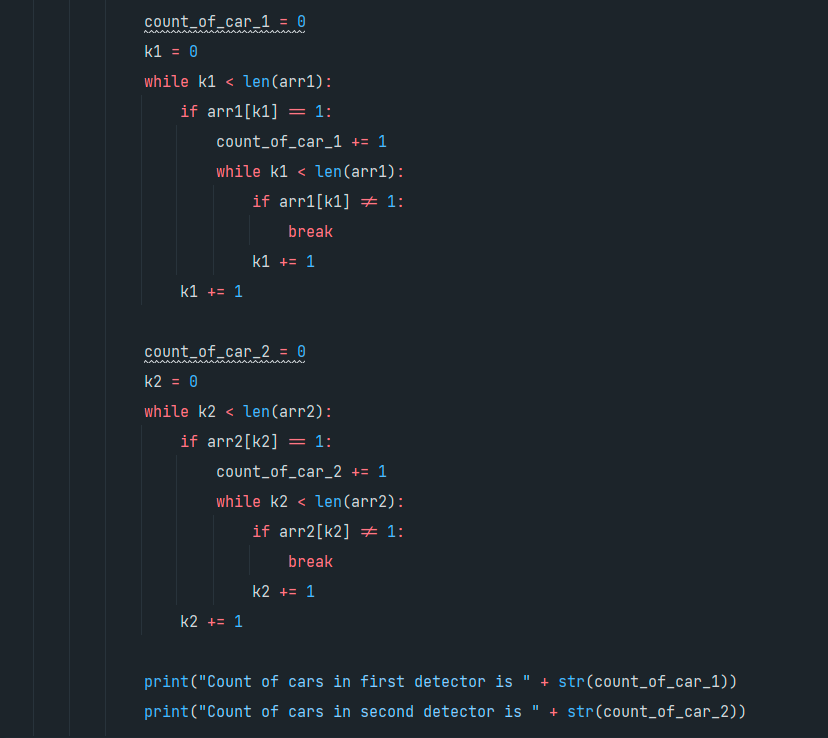
\includegraphics[width=0.8\linewidth]{car_count}
      \caption{количество машин в каждом из детекторов} 
      \label{} 
  \end{center} 
\end{figure}

\newpage

Использую полученные сведения о количестве проехавших машин через каждый детектор, а так же знаю время существования каждого детектора, можно расчитать интенсивность потока, за время работы видео.Результат приведён на рис.10.

\begin{figure}[h!]
  \begin{center}
      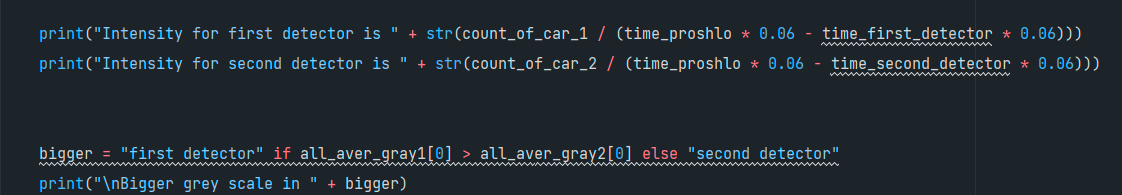
\includegraphics[width=0.8\linewidth]{intensity}
      \caption{Расчёт интенсивности потока для каждого детектора} 
      \label{} 
  \end{center} 
\end{figure}

\newpage  

\section*{Заключение}
В ходе выполнения данной работы был использован метод виртуальных детекторов. Этот метод позволяет оценивать количество автомобилей и интенсивность транспортного потока. 

\newpage 

\addcontentsline{toc}{section}{Список литературы} 
\begin{thebibliography}{}
  \bibitem{1}
  Методическое пособие "Latex2 - оформление документа"
  \bibitem{2}
  Документация Python https://docs.python.org/3/index.html

  
\end{thebibliography}

\newpage 

\section*{Приложение}

\begin{verbatim} 
import cv2
import numpy as np
import matplotlib.pyplot as plt


MAX_DETECTORS = 2
coord = []
all_aver_gray1 = []
all_aver_gray2 = []
size_of_decorator = 10
time_proshlo = 0
time_first_detector = 0
time_second_detector = 0


def discret(arr):
    listt = []
    for i in range(len(arr)):
        if i == 0:
            listt.append(0)
        elif (arr[0] - arr[i]) > arr[0] * 3 / 100:
            listt.append(1)
        else:
            listt.append(0)

    for i in range(0, len(listt) - 2):
        if listt[i] == 1 and listt[i + 2] == 1:
            listt[i + 1] = 1

    for i in range(0, len(listt) - 3):
        if listt[i] == 1 and listt[i + 3] == 1:
            listt[i + 1] = 1
            listt[i + 2] = 1

    for i in range(0, len(listt) - 3):
        if listt[i] == 0 and listt[i + 3] == 0:
            listt[i + 1] = 0
            listt[i + 2] = 0

    return listt


def add_coord(event, x, y, flags, param):

    global MAX_DETECTORS, ghf, time_first_detector, time_proshlo, time_second_detector

    if event == cv2.EVENT_LBUTTONDOWN:

        if len(coord) == 0 and time_first_detector == 0:
            time_first_detector = time_proshlo
        elif time_second_detector == 0:
            time_second_detector = time_proshlo

        if len(coord) >= MAX_DETECTORS:
            coord[0] = coord[1]
            del coord[1]
            coord.append((x, y))
        else:
            coord.append((x, y))

        ghf = True


def frame_capture(path):

    global coord, time_proshlo, time_first_detector, time_second_detector

    fig1, (ax1, ax2) = plt.subplots(nrows=1, ncols=2)
    ax1.set_title("first")
    ax1.set_ylim(0, 2)
    ax1.set_xlabel("Кадры")
    ax1.set_ylabel("")

    ax2.set_title("second")
    ax2.set_ylim(0, 2)
    ax2.set_xlabel("Кадры")
    ax2.set_ylabel("")
    fig1.suptitle("Бинаризированный график для каждого детектора")

    fig2, (ax3, ax4) = plt.subplots(nrows=1, ncols=2)
    ax3.set_title("first")
    ax3.set_ylim(80, 160)
    ax3.set_xlabel("Кадры")
    ax3.set_ylabel("Значение серого")

    ax4.set_title("second")
    ax4.set_ylim(80, 160)
    ax4.set_xlabel("Кадры")
    ax4.set_ylabel("Значение серого")
    fig2.suptitle("График значения серого цвета")

    fig3, (ax5, ax6) = plt.subplots(nrows=1, ncols=2)
    ax5.set_title("first")
    ax5.set_ylim(80, 160)
    ax5.set_xlabel("Секунды")
    ax5.set_ylabel("Значение серого")

    ax6.set_title("second")
    ax6.set_ylim(80, 160)
    ax6.set_xlabel("Секунды")
    ax6.set_ylabel("Значение серого")

    fig3.suptitle("График среднего цвета по времени")

    backsub = cv2.createBackgroundSubtractorMOG2()

    capture = cv2.VideoCapture(path) # path = video.mp4

    if capture:
        count_of_frame = 0
        while True:
            ret, frame = capture.read()  # Получаем сам кадр
            if ret:
                count_of_frame += 1
                cv2.namedWindow('Track')
                cv2.setMouseCallback('Track', add_coord)  # Связываем нажатие мыши с функцией

                gray = cv2.cvtColor(frame, cv2.COLOR_BGR2GRAY)

                # Находим объекты
                ret, gb = cv2.threshold(gray, 128, 255, cv2.THRESH_BINARY)
                gb = cv2.bitwise_not(gb)
                fgmask = backsub.apply(gray)  # Убираем фон
                contours, _ = cv2.findContours(fgmask.copy(), cv2.RETR_CCOMP, cv2.CHAIN_APPROX_SIMPLE)

                for i in range(len(coord)):  # Рисуем прямоугольник от нажатия мыши
                    cv2.rectangle(gray, (coord[i][0] - size_of_decorator, coord[i][1] - size_of_decorator),
                                  (coord[i][0] + size_of_decorator, coord[i][1] + size_of_decorator), (255, 0, 255), 2)

                    crop_image = gray[coord[i][1] - size_of_decorator:coord[i][1] + size_of_decorator, coord[i][0] - 30:coord[i][0] + size_of_decorator]
                    average_color_row = np.average(crop_image, axis=0)
                    average_color = int(np.average(average_color_row, axis=0))

                    if i == 0:
                        aver_gray1 = average_color
                        all_aver_gray1.append(aver_gray1)
                    else:
                        aver_gray2 = average_color
                        all_aver_gray2.append(aver_gray2)

                cv2.imshow("Track", gray)

            key = cv2.waitKey(60)
            time_proshlo += 1
            if key == ord('q'):
                length1 = min(count_of_frame, len(all_aver_gray1))
                length2 = min(count_of_frame, len(all_aver_gray2))

                arr1 = discret(all_aver_gray1)
                arr2 = discret(all_aver_gray2)

                ax1.plot(list(range(length1)), arr1[:length1])
                ax2.plot(list(range(length2)), arr2[:length2])

                ax3.plot(list(range(length1)), all_aver_gray1[:length1])
                ax4.plot(list(range(length2)), all_aver_gray2[:length2])

                len_1 = list()
                print(time_proshlo, time_first_detector, time_second_detector)
                for i in range(time_proshlo):
                    if i < time_first_detector:
                        len_1.append(0)
                    elif (i - time_first_detector) < len(all_aver_gray1):
                        len_1.append(all_aver_gray1[i - time_first_detector])
                    else:
                        len_1.append(0)

                len_2 = list()
                for i in range(time_proshlo):
                    if i < time_second_detector:
                        len_2.append(0)
                    elif (i - time_second_detector) < len(all_aver_gray2):
                        len_2.append(all_aver_gray2[i - time_second_detector])
                    else:
                        len_2.append(0)

                ax5.plot(list(map(lambda x: float(float(x) * 0.06), list(range(time_proshlo)))),
                         len_1)
                ax6.plot(list(map(lambda x: float(float(x) * 0.06), list(range(time_proshlo)))),
                         len_2)
                plt.show()

                count_of_car_1 = 0
                k1 = 0
                while k1 < len(arr1):
                    if arr1[k1] == 1:
                        count_of_car_1 += 1
                        while k1 < len(arr1):
                            if arr1[k1] != 1:
                                break
                            k1 += 1
                    k1 += 1

                count_of_car_2 = 0
                k2 = 0
                while k2 < len(arr2):
                    if arr2[k2] == 1:
                        count_of_car_2 += 1
                        while k2 < len(arr2):
                            if arr2[k2] != 1:
                                break
                            k2 += 1
                    k2 += 1

                print("Count of cars in first detector is " + str(count_of_car_1))
                print("Count of cars in second detector is " + str(count_of_car_2))

                print()

                print("Intensity for first detector is " + str(count_of_car_1 / (time_proshlo * 0.06 - time_first_detector * 0.06)))
                print("Intensity for second detector is " + str(count_of_car_2 / (time_proshlo * 0.06 - time_second_detector * 0.06)))


                bigger = "first detector" if all_aver_gray1[0] > all_aver_gray2[0] else "second detector"
                print("\nBigger grey scale in " + bigger)

                break


if __name__ == '__main__':
    frame_capture("video.mp4")
\end{verbatim}

\end{document}